\documentclass{article}

\usepackage{graphicx}
\usepackage{tikz}
\usepackage{tikzsymbols}
\usetikzlibrary{calc,patterns,shapes.geometric}
\pagestyle{empty}
\usepackage[margin=0pt]{geometry}
\geometry{papersize={14in,12in}}

\def\centerarc[#1](#2)(#3:#4:#5){\draw[#1] ($(#2)+({#5*cos(#3)},{#5*sin(#3)})$) arc (#3:#4:#5);}

\begin{document}
	\begin{figure}
		\centering
		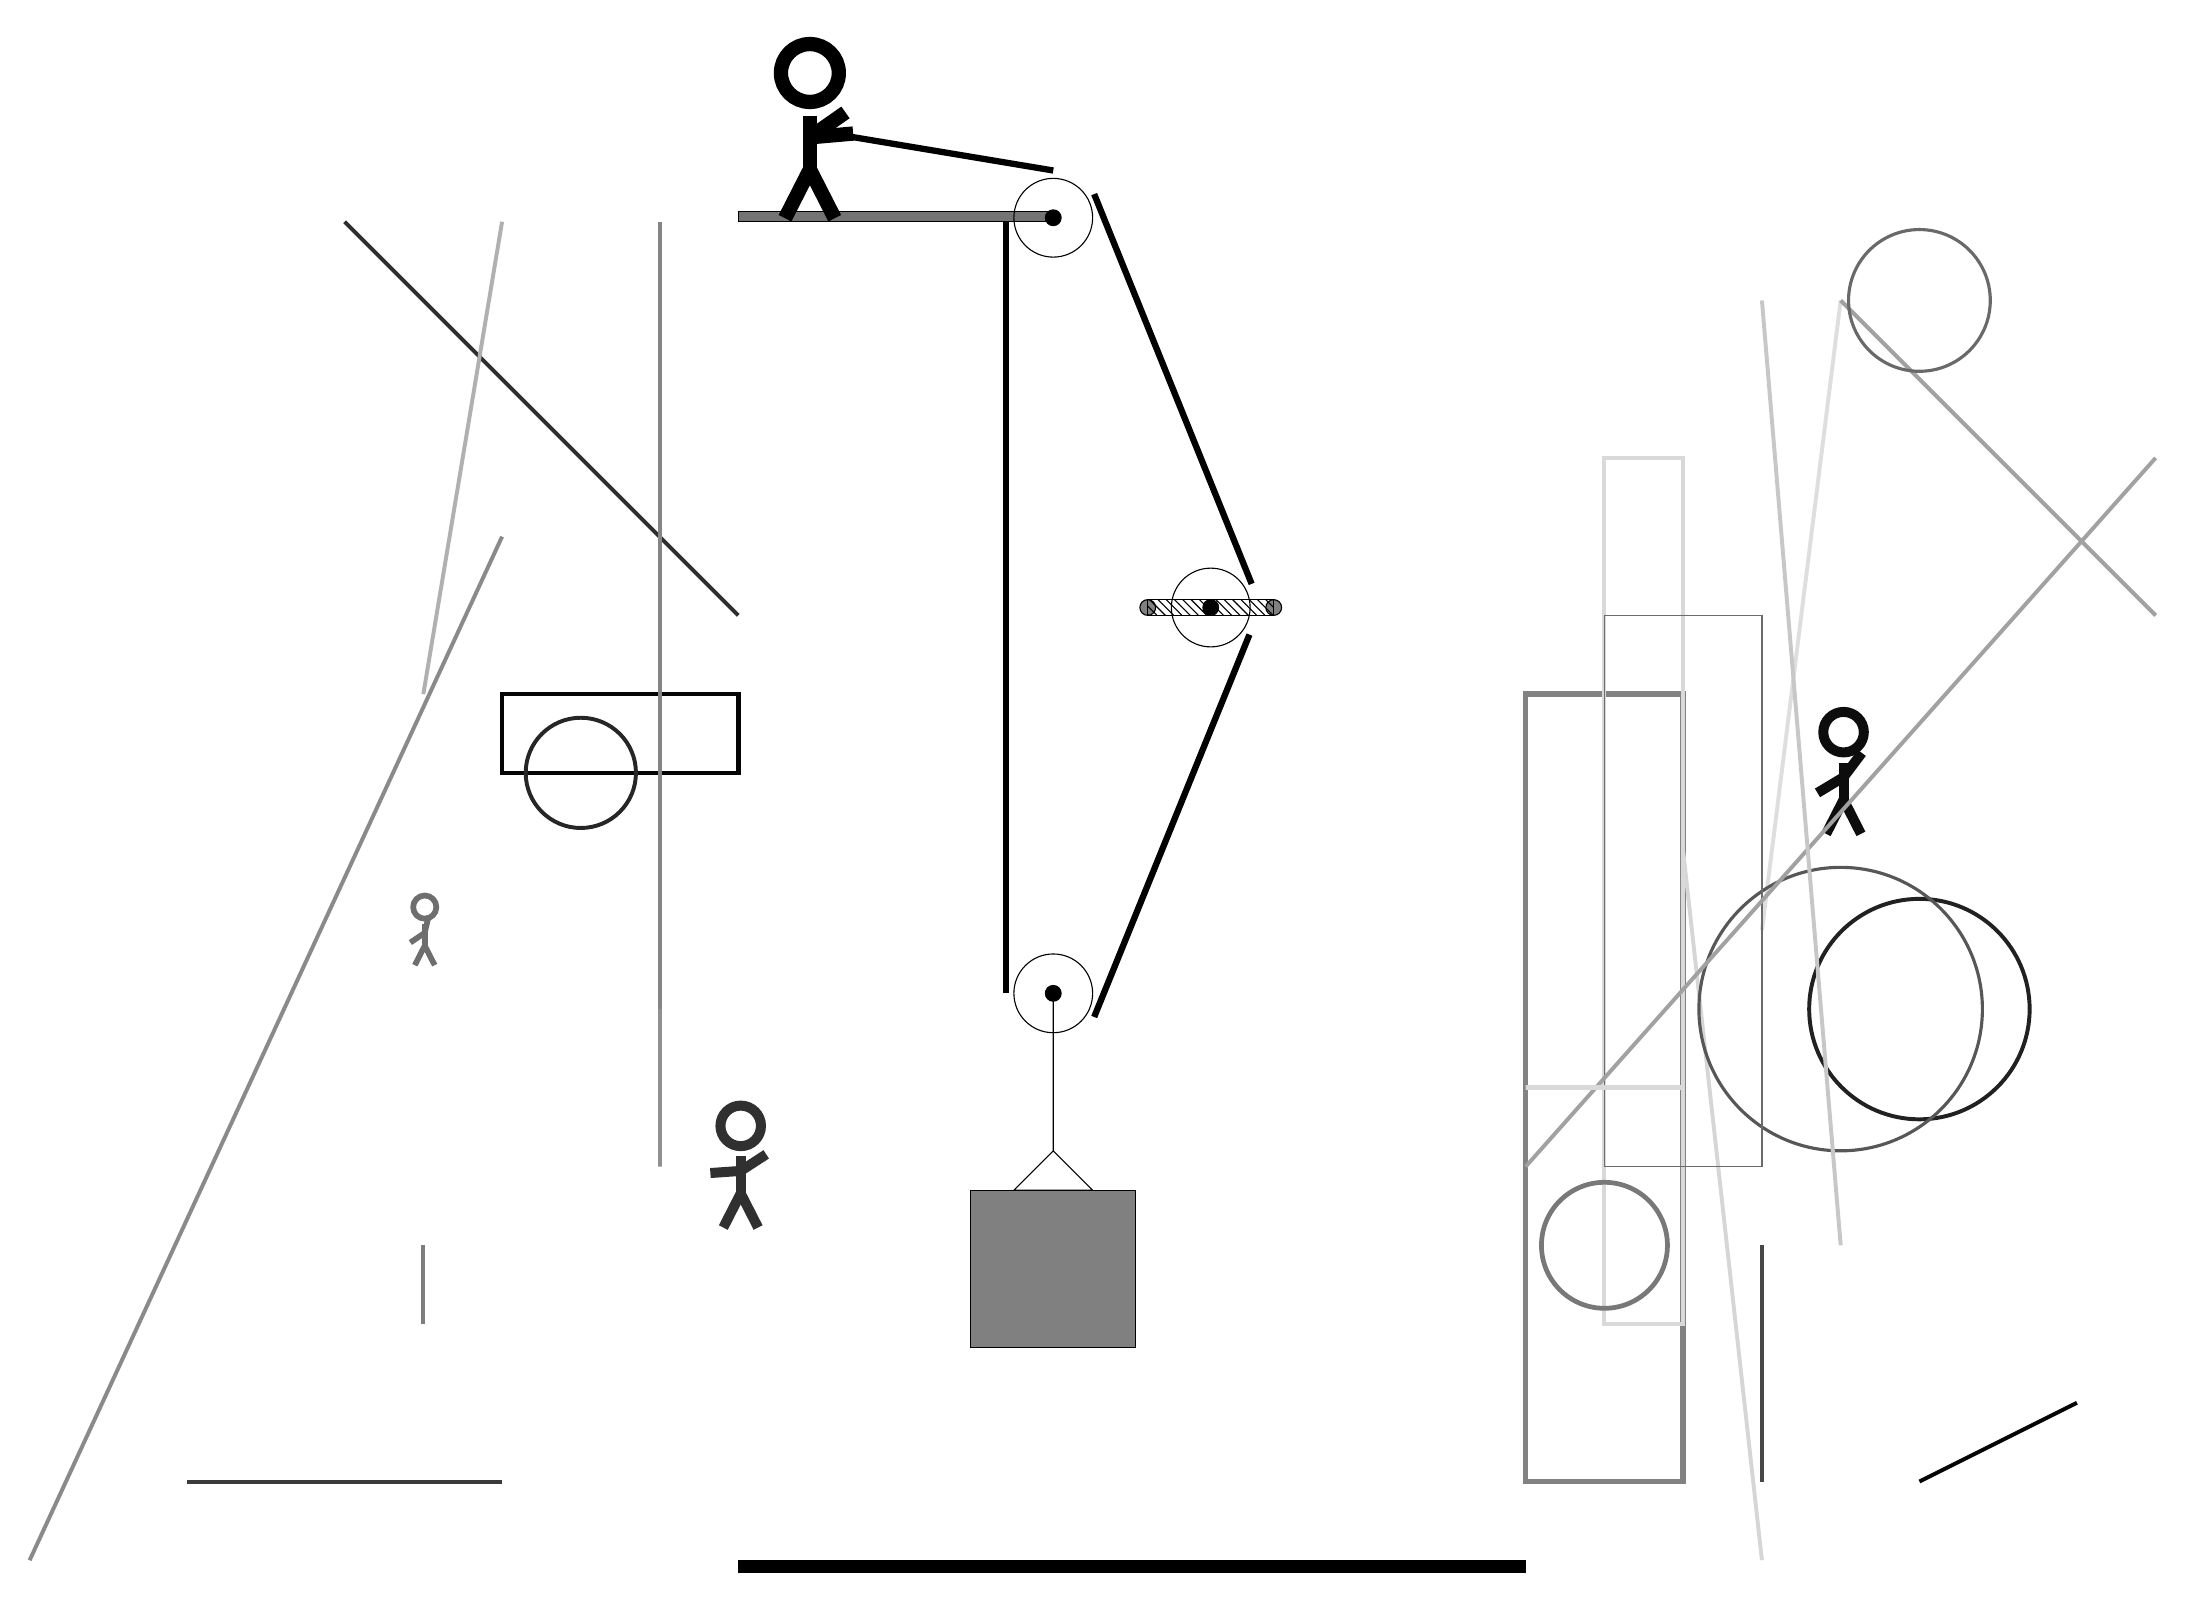
\begin{tikzpicture}
			%%%%% START %%%%%
			
			\draw[fill=black!55] (-2, 14) rectangle (2, 14.125);
			
			\draw (2, 4.2) circle (0.5);
			\draw[fill=black] (2, 4.2) circle (0.1);
			
			\draw (2, 14.05) circle (0.5);
			\draw[fill=black] (2, 14.05) circle (0.1);
			
			\draw[fill=white](4, 9.1) circle (0.5);
			\draw[fill=black] (4, 9.1) circle (0.1);
			\draw[fill=black!50] (3.2, 9.1) circle (0.1);
			\draw[fill=black!50] (4.8, 9.1) circle (0.1);
			\draw[pattern=north west lines, pattern color=black] (3.2, 9.2) rectangle (4.8, 9.0);
			
			\draw[line width=0.5mm, color=black!13](12, 13) -- (11, 5);
			
			\draw [line width=0.5mm, color=black!87](13, 4) circle (1.4);
			\draw[line width=0.5mm, color=black!37](12, 13) -- (16, 9);
			\draw[line width=0.6mm, color=black!98] (-2, 8) rectangle (-5, 7);
			\draw[line width=0.7mm, color=black!49] (8, 8) rectangle (10, -2);
			\draw[line width=0.5mm, color=black!82](-2, 9) -- (-7, 14);
			
			\draw[line width=0.5mm, color=black!46](-5, 10) -- (-11, -3);
			
			\draw[line width=0.5mm, color=black!77](-5, -2) -- (-9, -2);
			\draw[line width=0.5mm, color=black!16](11, -3) -- (10, 6);
			
			\draw[line width=0.5mm, color=black!15] (10, 0) rectangle (9, 11);
			
			\draw[line width=0.5mm, color=black!43] (-3, 5) rectangle (-3, 2);
			
			\draw [line width=0.6mm, color=black!53](9, 1) circle (0.8);
			\node[line width=0.2mm, color=black!95] at (12, 7) {\Strichmaxerl[7][31][53]};
			
			\draw [line width=0.4mm, color=black!66](12, 4) circle (1.8);
			\node[line width=0.4mm, color=black!81] at (-2, 2) {\Strichmaxerl[7][4][33]};
			\draw [line width=0.5mm, color=black!85](-4, 7) circle (0.7);
			\draw[line width=0.5mm, color=black!48](-3, 14) -- (-3, 4);
			
			\draw[line width=0.2mm, color=black!58] (9, 9) rectangle (11, 2);
			\node[line width=0.2mm, color=black!57] at (-6, 5) {\Strichmaxerl[4][34][77]};
			\draw [line width=0.4mm, color=black!59](13, 13) circle (0.9);
			\draw[line width=0.5mm, color=black!72](11, -2) -- (11, 1);
			
			\draw[line width=0.5mm, color=black!37](8, 2) -- (16, 11);
			\draw[line width=0.5mm, color=black!51](-6, 0) -- (-6, 1);
			\draw[line width=0.5mm, color=black!31](-6, 8) -- (-5, 14);
			\draw[line width=0.5mm, color=black!22](11, 13) -- (12, 1);
			
			\draw[line width=0.5mm, color=black!98](13, -2) -- (15, -1);
			\draw[line width=0.6mm, color=black!15] (8, 3) rectangle (10, 3);
			
			\draw (2, 4.2) -- (2, 2.2) -- (1.5, 1.7) -- (2.5, 1.7) -- (2, 2.2);
			\draw[fill=black!50] (0.95, 1.7) rectangle (3.05, -0.3);
			
			\draw[line width=0.8mm] (1.4, 14) -- (1.4, 4.2);
			\centerarc[line width=0.8mm](2, 4.2)(180:330:0.6);
			\draw[line width=0.8mm](2.5196, 3.9) -- (4.4915, 8.7558);
			\centerarc[line width=0.8mm](4, 9.1)(390:325:0.6);
			\draw[line width=0.8mm](4.5196, 9.4) -- (2.5196, 14.35);
			\centerarc[line width=0.8mm](2, 14.05)(30:90:0.6);
			\draw[line width=0.8mm](2, 14.65) -- (-1, 15.15);
			
			\node at (-1, 15.15) {\Strichmaxerl[10][-175][35]};
			
			\draw[fill=black] (-2, -3) rectangle (8, -3.15);
			
			%%%%% END %%%%%
		\end{tikzpicture}
	\end{figure}	
\end{document}